
\chapter{Des Applications de SDN et leurs possibilités}

%Ce chapitre a pour but de présenter ce qui apporte SDN, quelles sont les applications pratiques de ce nouvel paradigme. Ce ne sera pas exhaustive, mais c'est pour exemplifier. Cela permettra aussi d'avoir une idée de l'exploitation future de SDN.

Une infinité d'applications et de cas d'utilisation sont imaginables. Ce chapitre propose d'analyser les enjeux auxquels on espère pouvoir répondre avec SDN et de présenter des applications plutôt ciblées sur ces expectatives. De cette analyse, les cas d'utilisation plus cohérents seront identifiés et ensuite détaillés.

 
%\section{Identifications des applications espérées par les utilisateurs}

%In August and September of 2013 a survey was given to the subscribers of Webtorials.
Entre les mois d'août et septembre de 2013, Webtorials a réalisé un sondage auprès de ses abonnés. Une des enquêtes a été sur les challenges et opportunités qu'ils pensent pouvoir adresser avec SDN au sein des organisations de \gls{ti} typiques. Le tableau 3.1 affiche le pourcentage de réponses positives pour chaque challenge. \cite{2013GuideSDNNVUseCases}

\begin{table}[!h]
\centering
\begin{tabular}{|p{12cm}|c|}
\hline 
\bf Challenge ou Opportunité & \bf Pourcentage \\ 
\hline 
Meilleure utilisation des ressources réseau & 51\% \\ 
\hline 
Simplifier la configuration de la QoS et de la sécurité  & 47\%  \\
\hline 
Réaliser l'ingénierie du trafic avec vision point-à-point du réseau & 44\% \\ 
\hline 
Évolution plus facile des fonctions réseau & 39\% \\ 
\hline 
Support dynamique au management de ressources virtuelles  & 38\% \\ 
\hline 
Établissement des réseaux Ethernet virtuels sans les contraintes du fardeau de configuration des VLANs & 35\% \\ 
\hline 
Réduction de la complexité & 34\% \\ 
\hline 
Permettre les demandes dynamiques de services au réseau & 32\% \\ 
\hline 
Réduction des dépenses d'exploitation & 30\% \\ 
\hline 
Faire évoluer les fonctionnalités réseau plus rapidement en s'appuyant sur les cycles de vie du développement logiciel & 27\% \\ 
\hline 
Implémentation plus facile de la QoS & 27\% \\ 
\hline 
Implémentation des fonctionnalités de sécurité plus efficaces & 26\% \\ 
\hline 
Réduction des dépenses d'investissement de capital & 25\% \\ 
\hline 
Absence de challenges/opportunités pouvant être adressés par SDN & 3\% \\ 
\hline 
\end{tabular}
\caption{Opportunités et Challenges adressés par SDN \cite{2013GuideSDNNVTable11}}
\end{table} 

\clearpage

De ces résultats on peut conclure que le marché compte pouvoir se bénéficier de SDN sur une vaste gamme de challenges et opportunités, c'est qui démontre des expectatives tout à fait favorables pour la technologie. Cette variété de sujets est en général intéressant pour l'adoption du \gls{paradigme} mais peut causer des confusions au début ralentissant les actions à ce moment-là.

Dans les même sondage les participants on répondu que si leurs organisations implémentent SDN dans les deux ans que suivent, il est plus probable que cela soit sur \gls{datacenter} (54\%), section et/ou campus (26\%), WAN (23\%) ou pas d'implémentation SDN (11\%) \cite{2013GuideSDNNVTable12}. Par conséquent, les applications présentées ci-après sont classées sur ces trois cibles de déploiement.




\section{Data Center}

\textbf{\glspl{vlan}}. SDN peut facilement fournir aux utilisateurs leurs propre réseaux isolés, comme les VLANs. L'approche la plus simple est de déclarer les ensembles de flux statiquement qui spécifient les ports accessibles par un VLAN ID donné. Le trafic identifié venant d'un type d'utilisateur (à l'origine d'un port du switch ou d'une adresse MAC spécifiés) est marqué dans le VLAND ID approprié. Une approche plus dynamique pourrait utiliser le contrôleur pour gérer l'authentification des utilisateurs et d'utiliser les informations sur leurs localisation pour marquer le trafic à la volée. \cite{OpenFlowStanfordUsing} 

%VLANs. OpenFlow can easily provide users with their own isolated network, just as VLANs do. The simplest approach is to statically declare a set of flows which specify the ports accessible by traffic on a given VLAN ID. Traffic identified as coming from a single user (for example, originating from specific switch ports or MAC addresses) is tagged by the switches (via an action) with the appropriate VLAN ID. A more dynamic approach might use a controller to manage authentication of users and use the knowledge of the users’ locations for tagging traffic at runtime.



%Most networking vendors offer data center fabric solutions featuring some form of Layer 2 multi-pathing to improve the networks capacity to handle “east-west” traffic flow characteristic of server virtualization, converged storage networking, and cluster computing. SDN provides an effective solution to this problem because the network path is determined by a central controller and does not require the use of STP. Thus, all inter-switch links can be fully utilized and traffic can be directed between multiple LANs without the need for first routing the traffic to higher-level switches.



\textbf{Raccordement réseau de deux data centers}. SDN permet de relier des réseaux au niveau de la couche 2 à travers des multiples data centers, les couvrant comme s'ils étaient dans un seul réseau. Avec cette fonctionnalité, les architectes d'applications peuvent par exemple placer leurs "compute clusters" dans leur point d'usage et supporter une efficace récupération après incident. \cite{ODCAusageScenarios}
%Data Center L2 Network Bridging. SDN enables bridging of Layer 2 networks across multiple data centers, providing a single overlay network. With this capability, application architects can place compute clusters closer to their point of usage and support effective disaster recovery.

\begin{figure}[!h] %on ouvre l'environnement figure
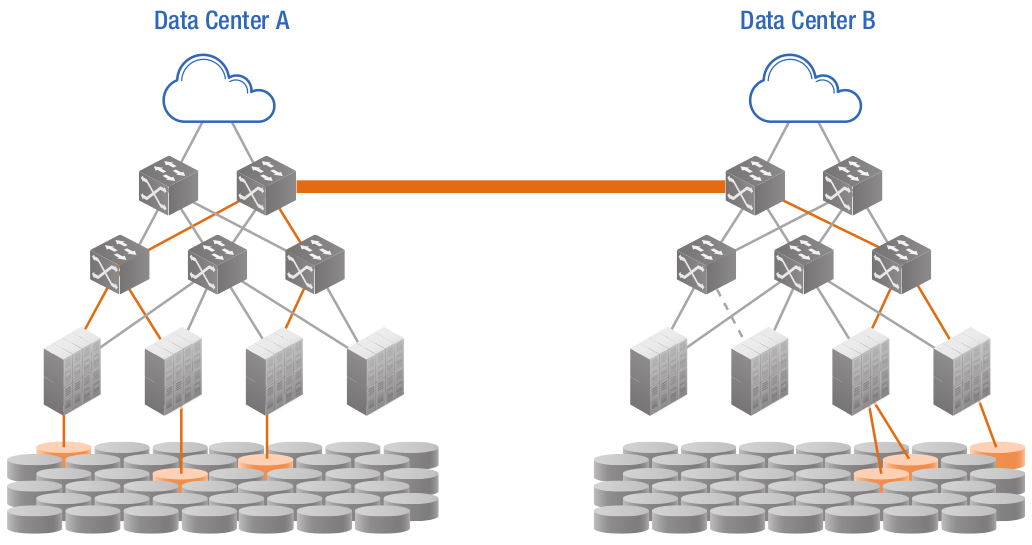
\includegraphics[width=15cm]{images/DataCenterL2Bridging.png} %ou image.png, .jpeg etc.
\caption{ Raccordement réseau de deux Data Centers \cite{ODCAusageScenarios}} %la légende
\label{imgDCL2B} %l'étiquette pour faire référence à cette image
\end{figure} %on ferme l'environnement figure

\textbf{Répartition de charge et sécurité}. FlowScale est une application basée sur OpenFlow qui fourni la répartition de charge du trafic réseau en utilisant du switch OpenFlow. L'application a été utilisé dans un système \gls{ids} pour distribuer le trafic uniformément aux senseurs. Quand complètement déployé, le système sera capable de distribuer le trafic à de taux dépassant 500Gb/s.  \cite{FlowScale}
%Indiana University has developed an OpenFlow-based, load-balancing application called FlowScale. According to the University 15, “FlowScale provides complex, distributed load balancing of network traffic using an OpenFlow-capable Top of Rack (ToR) switch. IU deployed the application into its Intrusion Detection System (IDS) to distribute traffic evenly to sensors. When fully deployed, the system will span the IU Bloomington and IUPUI networks and have the capability to distribute traffic at rates exceeding 500Gb/s.”

%\bf{Monitoring Réseau}. Avec SDN, la redirection de flux réseau peut être programmée, permettant de surveiller le trafic sélectionne sans le rediriger physiquement.  
%Network Taps. With OpenFlow virtual ports, the functionality of a network tap can be programmed into the OpenFlow switch, allowing selected traffic to be monitored without deploying physical taps. Traffic can also be replicated and redirected to any monitoring device in the network. Big Switch networks has announced such a network monitoring application referred to as Big Tap 16.

\textbf{Economie d'énergie}. ElasticTree est un gestionnaire d'énergie pour le réseau. Le projet utilise SDN pour trouver la configuration réseau plus économique qui satisfait les conditions de trafic en éteignant les équipements qui ne sont pas nécessaires. Le projet a obtenu des économies d'énergie entre 25 et 62\% sous diverses conditions de trafic \cite{ElasticTree}. Ces économies peuvent être augmentées en introduisant la virtualisation et la gestion des serveurs. Une possibilité est le travail Honeyguide qui propose une optimisation d'énergie en utilisant la migration de \glspl{vm} pour augmenter la quantité de \glspl{vm} et de switches pouvant être arrêtés \cite{Honeyguide}.


%They proposed ElasticTree, a network-wide power manager that utilizes SDN to find the minimum-power network subset which satisfies current traffic conditions and turns off switches that are not needed. As a result, they show energy savings between 25-62\% under varying traffic conditions. One can imagine that these savings can be further increased if used in parallel with server management and virtualization; one possibility is the Honeyguide[80] approach to energy optimization which uses virtual machine migration to increase the number of machines and switches that can be shutdown.


\textbf{Applications sur Cloud Computig}. Dans les offres \gls{iaas}, les utilisateurs ont une vision et un contrôle du réseau  limités. Les technologies SDN peuvent faciliter la délégation de contrôle du réseau et fournir certains niveaux d'abstraction aux utilisateur finaux leurs permettant de configurer leur morceau du réseau. De plus, les offres clouds basées sur SDN pourront fournir des services de bande passante sous demande avec la provision automatisée et intelligente, dirigés par une logique d'orchestration cloud et par les besoins des clients. \cite{AdoptionResearchTrendsCloud}

%Offering Infrastructure as a Service (IaaS), users only get a logical view of the underlying network and have limited control. SDN technologies have the capabilities to facilitate delegation of network controls and provide some level of network abstractions to end-users to enable them to configure their slice of the network. Delegating more control to the end-users could raise security concerns for the providers [Azodolmolky13]. SDN-based clouds will allow enterprises to have multi-vendor networks to avoid vendor lock-in. They can access dynamic bandwidth for ad- hoc, timely inter-data center workload migration and processing; and eliminate the burden of underutilized, costly high-capacity fixed private leased lines. SDN-enabled bandwidth-on-demand services provide automated and intelligent service provisioning, driven by cloud service orchestration logic and customer requirements.



\section{Campus et grands réseaux}

Souvent les entreprises opérant des grands réseaux ont des requis strictes de performance et sécurité qui peuvent varier largement selon divers facteurs. Par exemple, les réseaux des universités sont considérés comme un cas spécial des réseaux d'entreprises : dans cet environnement, plusieurs dispositifs connectés sont temporaires et ne sont pas contrôlés par l'institution, en outre mettant en question la sécurité et l'allocation de ressources. L'adéquation du management est critique dans ces conditions et SDN peut être utilisé pour imposer et ajuster les politiques réseaux par programmation ainsi qu'aider à surveiller l'activité et régler la performance.

%Enterprises often run large networks, while also having strict security and performance requirements. Furthermore, different enterprise environments can have very different requirements, characteristics, and user population, For example, University networks can be considered a special case of enterprise networks: in such an environment, many of the connecting devices are temporary and not controlled by the University, further challenging security and resource allocation. Additionally, Universities must often provide support for research testbeds and experimental protocols. Adequate management is critically important in Enterprise environments, and SDN can be used to programmatically enforce and adjust network policies as well as help monitor network activity and tune network performance.

\textbf{Management du réseau et contrôle d'accès}.
Une implémentation d'un contrôleur, adaptée pour le management et contrôle du réseau, qui gère l'admission et le routage des flux. L'idée de base est de permettre aux administrateurs réseaux de définir des politiques applicables à tout le réseau dans un contrôleur central. Ces politiques seront renforcés directement par la réalisation du contrôle d'admission sur le traitement de chaque nouveau flux. Le contrôleur vérifie que le nouveau est en conformité avec un ensemble de règles, tels que "les hôtes peuvent communiquer via \gls{http} seulement passant par un proxy" ou "téléphones VoIP ne sont pas autorisés à communique avec les laptops". Un contrôleur associe des paquets avec leur émetteurs avec la liaison entre noms et adresses, basique-ment il prend le contrôle du \gls{dns} et du \gls{dhcp} et authentifie tous les utilisateurs qui se rejoignent, gardant trace des ports de switches ou point d'accès utilisé pour la connexion.

%Network Management and Access Control. An implementation of a controller, suited for network management and control, that manages the admittance and routing of flows. The basic idea is to allow network managers to define a Controller network-wide policy in the central controller, which is enforced directly by making admission control decisions for each new flow. A controller checks a new flow against a set of rules, such as “Guests can communicate using HTTP, but only via a web proxy” or “VoIP phones are not allowed to communicate with laptops.” A controller associates packets with their senders by managing all the bindings between names and addresses — it essentially takes over DNS, DHCP and authenticates all users when they join, keeping track of which switch port (or access point) they are connected to. \cite{OpenFlowStanfordUsing}

\textbf{Connexion sans fils mobile}.
Plusieurs efforts ont été focalisés dans la connectivité omniprésente dans le contexte des infrastructures basées sur l'accès sans fil au réseau, comme le WiFi. Par exemple, des expériences ont été faites pour les clients mobiles VoIP sur la proposition d'un nouveau mécanisme de transfert d'appel. Un contrôleur est implémenté pour tracer la localisation des clients et être capable de re-router les connexions (avec la re-programmation des tableaux de flux) au moment où les utilisateurs se déplacent dans le réseau. Cela permettra le transfert transparent d'un point d'accès à l'autre sans coupure de l'appel. \cite{OpenFlowStanfordUsing}

%Infrastructure-based Wireless Access Networks. Several efforts have focused on ubiquitous connectivity in the context of infrastructure-based wireless access networks,such as cellular and WiFi.
%Mobile wireless VOIP clients. For this example consider an experiment of a new call-handoff mechanism for WiFi-enabled phones. In the experiment VOIP clients establish a new connection over the OpenFlow-enabled network. A controller is implemented to track the location of clients, re-routing connections — by reprogram-ming the Flow Tables — as users move through the network, allowing seamless handoff from one access point to another. \cite{OpenFlowStanfordUsing}


\section{WAN}
Dans un \glspl{wan}, la centralisation permet le calcul déterministe et optimal de routes pour chaque flux avec l'utilisation d'un model complet de la topologie bout-en-bout du réseau. L'allocation de bande passante peut être contrôlé dynamiquement pour fournir à la demande lors des changements de trafic. Le résultat peut être une meilleure utilisation du réseau sans sacrifier la qualité de service. Le traitement centralisé de route permet aussi de pré-déterminer les routes alternatives pour chaque lien en cas de failles. On peut profiter de la puissance de traitement des processeurs à multiples cœur et les \glspl{cluster} pour le calcul de routes et le traitement de nouveaux flux. Cette application correspond à une de trois plus espérées pour le marché. \cite{2013GuideSDNNVUseCases}


%Centralization allows optimum routes to be calculated deterministically for each flow by leveraging a complete model of the end-to-end topology of the network. Bandwidth allocations can be controlled dynamically to provide bandwidth on demand with changing traffic patterns. The result can be much better utilization of the network without sacrificing service quality. Centralized route processing also allows the pre-computation of a set of fail-over routes for each possible link or node failure. Centralized processing also can take advantage of the virtually unlimited processing power of multi-core processors and cluster computing for calculating routes and processing new flows. As shown in Table 11, being able to do end-to-end traffic engineering is one of the top three opportunities that The Survey Respondents associate with SDN.



Avec SDN, le trafic WAN peut être dynamiquement re-routé pour réduire/contôler la latence pour les applications sensibles, comme VoIP. La charge du trafic peut être également repartie sur des chemins parallèles à différents coûts.
%WAN traffic can be dynamically rerouted to reduce/control latency for VoIP and other latency sensitive applications. Traffic can also be load balanced over parallel paths of differing costs.
Des métriques des flux temps réel peuvent être utilisés pour la limiter le débit ou modifier la transmission optimisant la performance des applications. Par exemple, le contrôleur peut configurer un switch compatible pour modifier les marquage QoS pour changer les priorités sur les chemins point-à-point restants.
%With OpenFlow V 1.3, per flow meters can be used for rate limiting or to provide real time visibility of application performance allowing the controller to modify forwarding behavior to maximize application performance. For example, the controller can configure an OpenFlow switch to modify the QoS markings to change the priority received over the remainder of the end-to-end path.
La récupération des liens échoués peut être atteinte avec la sélection dynamique de chemins, tenant compte des métriques de performance, les états de ports et niveaux d'utilisations par les nœuds.
%With extensions in V1.3 and V1.4, OpenFlow can support circuit-switched paradigms, including CWDM, DWDM, and MPLS with specific path selection and requested levels of CBR and priority. Circuits can be provisioned on a dynamic, scheduled, or permanent basis. Recovery from failed circuits can be via predetermined backup paths or by dynamic path selection. Circuit provisioning can take into account performance metrics, port states, and endpoint utilization.

Un exemple pratique d'une application réelle de SDN a été présenté par Google. L'entreprise a présenté dans la conférence "Open Network Summit" \cite{googleONS} une implémentation à grande échelle d'un réseau SDN connectant des \glspl{datacenter} partout dans le monde. Le travail, intitulé B4 \cite{SDNWANB4}, présente en détails la conception, implémentation et évaluation de ce WAN connectant les \glspl{datacenter} Google géographiquement distribués. Le travail décrit un de premiers et plus grands déploiements SDN. Sa motivation a été le besoin pour des routes et ingénierie du trafic personnalisées ainsi que le haut niveau de "scalability", tolérance aux failles, rentabilité et contrôle requis et ne pouvant pas être accomplis avec l'architecture WAN traditionnelle. La solution a proposée une architecture SDN basée sur OpenFlow construite pour contrôle des switches particuliers. Après trois en production, B4 se montre efficace dans le sens qu'il dirige des nombreux liens avec une utilisation près de 100\% et au même temps partageant les flux sur des multiples chemins. \cite{SurveySDNApplications}


%A practical example of a real application of the SDN concept and architecture in the context of data centers was presented by Google in early 2012. The company presented at the Open Network Summit [81] a large scale implementation of an SDN-based network connecting its data centers. The work in [82] presents in more detail the design, implementation, and evaluation of B4, a WAN connecting Google’s data centers world wide. This work describes one of the first and largest SDN deployments. The motivation was the need for customized routing and traffic engineering and the fact that the level of scalability, fault tolerance, cost efficiency and control required, could not be achieved by means of a traditional WAN architecture. A customized solution was proposed and an OpenFlow-based SDN architecture was built to control individual switches. After three years in production, B4 is shown to be efficient in the sense that it drives many links at near 100\% utilization while splitting flows among multiple paths. Furthermore, the experience reported in the work shows that the bottleneck resulting from control-plane to data-plane communication and overhead in hardware programming are important issues to be considered in future work. 



%\section{Management du Réseau et Contrôle d'Accès}
%Association des flux aux groupe d'utilisateur permettant de définir les politiques d'accès à différents services.

%\section{VLANs}
%Réseaux isolés définis par flux.

%\section{Clients mobiles sans fil VoIP}


